\chapter{平面与平面系统}

\begin{introduction}
	\item 平行平板(第 \ref{sect:parallel-plate} 节)
	\item 常见的反射棱镜(第 \ref{sect:reflecting-prism} 节)
	\item 最小偏折角(式(\ref{eq:minimum-deviation-angle}))
	\item 阿贝常数与色散(第 \ref{sect:optical-material} 节)
\end{introduction}

\section{平面镜成像}
平面镜即平面反射镜,由式(\ref{eq:spherical-refraction}),在平面镜成像中,有

\begin{equation}
l'=-l,\quad\beta=1
\end{equation}
物与像分别位于镜面的两侧,且到镜面的距离相等,平面镜成正立,与物同等大小的像。平面镜对食物成虚像,对虚物成实像。

为了避免成像产生镜像,光学仪器中需要采用偶数个镜面。如\figref{fig:one-mirror} 所示,当入射光线方向不变而转动平面镜时,反射光线的方向将发生改变,平面镜转过$\alpha$角度时,反射光线将转过$2\alpha$角。如\figref{fig:two-mirror} 所示,光线经双平面镜两个面相继反射一次后的出射光线$\beta$与两个面的夹角$\alpha$之间存在关系

\begin{equation}
\beta=2(I_1+I_2)=2\alpha
\end{equation}
即出射光线与入射光线的夹角是双镜夹角$\alpha$的$2$倍。

\begin{figure}[htbp]
	\centering
	\begin{minipage}[t]{0.48\textwidth}
		\centering
		\begin{tikzpicture}
		\draw[-latex] (0:0) -- (5:2.5);
		\draw[latex-] (0:0) -- (135:2.5);
		\draw[-latex] (0:0) -- (45:2.5);
		\draw[-] (0:0) -- (90:2.5);
		\draw[-] (0:0) -- (70:2.5);
		\draw[-] (180:2.5) -- (0:2.5);
		\draw[-] (160:2.5) -- (-20:2.5);
		\filldraw[pattern=north east lines] (180:2.5) -- (0:2.5) -- (-1:2.5) -- (181:2.5) -- (180:2.5);
		\filldraw[pattern=north east lines] (160:2.5) -- (-20:2.5) -- (-21:2.5) -- (161:2.5) -- (160:2.5);
		\draw[-latex] (-0.8,0) arc (180:160:0.8);
		\draw[-latex] (0,0.8) arc (90:70:0.8);
		\draw[-latex] (0.3535,0.3535) arc (45:5:0.5);
		\node[] at (170:1.1) {$\alpha$};
		\node[] at (80:1.1) {$\alpha$};
		\node[] at (25:0.9) {$2\alpha$};
		\node[] at (90:2.6) {$N$};
		\end{tikzpicture}
		\caption{单平面镜对光的变换}
		\label{fig:one-mirror}
	\end{minipage}
	\quad
	\begin{minipage}[t]{0.48\textwidth}
		\centering
		\begin{tikzpicture} 
		\coordinate (A) at (-1.299,3);
		\coordinate (B) at (150:1.5);
		\coordinate (C) at (90:1.5);
		\coordinate (D) at (120:1.732);
		\coordinate (E) at (-0.75,1.5);
		\coordinate (F) at (-1.299,2.25);
		\draw[-] (0:0) -- (90:3);
		\draw[-] (0:0) -- (150:3);
		\filldraw[pattern=north east lines] (0:0) -- (90:3) -- (89:3) -- (0:0.05) -- (0:0);
		\filldraw[pattern=north east lines] (0:0) -- (150:3) -- (151:3) -- (240:0.05) -- (0:0);
		\draw[latex-] (150:1.5) -- (-1.299,3);
		\draw[-latex] (150:1.5) -- (90:1.5);
		\draw[latex-] (-2.598,3) -- (90:1.5);
		\draw[-] (180:1.732) -- (120:1.732);
		\draw[-] (-0.75,1.5) -- (0.75,1.5);
		\node[] at (150:3.3) {$M_1$};
		\node[] at (90:3.2) {$M_2$};
		\node[] at (180:2) {$N_1$};
		\node[] at (1,1.5) {$N_2$};
		\draw[-] (0,0.4) arc (90:150:0.4);
		\node[] at (120:0.6) {$\alpha$};
		\pic["$I_1$", draw=black, -, angle eccentricity=1.3, angle radius=0.5cm] {angle=D--B--A};
		\pic["$I_2$", draw=black, -, angle eccentricity=1.3, angle radius=0.5cm] {angle=E--C--B};
		\pic["$\beta$", draw=black, -, angle eccentricity=1.6, angle radius=0.3cm] {angle=C--F--A};
		\end{tikzpicture}
		\caption{双平面镜对光的变换}
		\label{fig:two-mirror}
	\end{minipage}
\end{figure}

\begin{problem}
	夹角为$35$度的双平面镜系统,当光线以多大的入射角入射于一平面镜时,其反射光线再经另一平面镜反射后,将沿原光路反向射出?
\end{problem}
\begin{solution}
	由\figref{fig:two-mirror} 所示的图像可以看出,若要使光线原路反射,需要垂直入射到第二个平面镜上。根据几何关系可知,入射角为$35$度。
\end{solution}

\begin{problem}
	有一双平面镜系统,光线与其中的一个镜面平行入射,经两次反射后,出射光线与另一镜面平行,问二平面镜的夹角是多少?
\end{problem}
\begin{solution}
	设双平面镜夹角为$\alpha$,由\figref{fig:two-mirror} 所示的图像可以看出,入射光与出射光的夹角为$\alpha$和$2\alpha$,则有$\alpha+2\alpha=180^{\circ}$,得$\alpha=60^{\circ}$。
\end{solution}

\section{平行平板}
\label{sect:parallel-plate}

逐面应用折射球面物像公式(\ref{eq:spherical-refraction}),考虑到$r_1=r_2=\infty$,可得
\begin{equation}
l'=nl,\quad l_2=nl-d,\quad l'=l-\frac{d}{n}
\end{equation}
\begin{equation}
\beta=\beta_1\beta_2=1
\end{equation}
式中$n$和$d$为平行平板的折射率和厚度。

\begin{definition}{平行平板}{parallel-plate}
	由两个相互平行的折射平面构成的光学器件称为平行平板
\end{definition}

\begin{property}
如\figref{fig:parallel-plate-1} 所示,平行平板总对物成同等大小的正立像,物与像总在平板同侧,两者虚实不一致。不论物距为何值,像相对于物的位置总不改变
\end{property}

像相对于物的距离为
\begin{equation}
\Delta l'=-l+d-(-l')=d\bigg(1-\frac{1}{n}\bigg)
\end{equation}
$\Delta l'$恒为正值,所以平行平板所成像总是由物沿光线前进方向沿轴移动$d(1-1/n)$得到,和物的位置、虚实无关。

\begin{figure}[htbp]
	\centering
	\begin{minipage}[t]{0.48\textwidth}
		\centering
		\begin{tikzpicture}[scale=0.9] 
		\draw[-] (-3.5,0) -- (3.5,0);
		\draw[-,name path=pathA] (3,-2) -- (3,2);
		\draw[-,name path=pathB] (2,-2) -- (2,2);
		\draw[-,dashed,name path=pathC] (-3,0) -- (3,1.5);
		\path [name intersections={of = pathB and pathC, by=B}];
		\path [name intersections={of = pathA and pathC, by=C}];
		\draw[-latex,red] (-0.5,0) -- (2,1.25);
		\draw[-,dashed] (0,0) -- (3,1.5);
		\draw[-latex,red] (B) -- (C);
		\draw[-latex,red] (3,1.5) -- (3.5,1.75);
		\node[] at (-0.8,-0.2) {$A$};
		\node[] at (0.2,-0.2) {$A'$};
		\node[] at (2.5,-1) {$n$};
		\coordinate (A) at (0,0);
		\coordinate (D) at (-0.5,0);
		\pic["$-U$", draw=black, -, angle eccentricity=1.6, angle radius=0.6cm] {angle=A--D--B};
		\draw[-] (-0.5,0) -- (-0.5,-2);
		\draw[-] (0,0) -- (0,-1.5);
		\draw[latex-latex](0,-1.2) -- (3,-1.2) node[black,above,midway](line){$-l'$};
		\draw[-latex](-1,-1.2) -- (-0.5,-1.2);
		\node[] at (-0.75,-0.9) {$\Delta l'$};
		\draw[latex-latex](2,-1.7) -- (3,-1.7) node[black,above,midway](line){$d$};
		\draw[latex-latex](2,-1.7) -- (-0.5,-1.7) node[black,above,midway](line){$-l$};
		\end{tikzpicture}
		\caption{平行平板成像(一)}
		\label{fig:parallel-plate-1}
	\end{minipage}
	\quad
	\begin{minipage}[t]{0.48\textwidth}
		\centering
		\begin{tikzpicture}[scale=0.9] 
		\draw[-] (-3.5,0) -- (4,0);
		\draw[-] (3,-2) -- (3,2);
		\draw[-] (1,-2) -- (1,2);
		\draw[-] (0,1) -- (3,1);
		\draw[-] (2,1.25) -- (4,1.25);
		\draw[-] (-3,0) -- (-3,-2);
		\draw[-] (-2,0) -- (-2,-2);
		\coordinate [label=above:$A$](A) at (-3,0);
		\coordinate [label=above left:$D$](B) at (1,1);
		\coordinate [label=below right:$A'$](C) at (-2,0);
		\coordinate [label=below right :$E$](D) at (3,1.25);
		\coordinate (E) at (4,1.5);
		\coordinate (F) at (3,0);
		\coordinate (G) at (0,1);
		\coordinate (H) at (3,1);
		\coordinate (I) at (2,1.25);
		\coordinate (J) at (4,1.25);
		\draw[-latex,red] (A) -- (B);
		\draw[-,dashed] (C) -- (D);
		\draw[-latex,red] (B) -- (D);
		\draw[-latex,red] (D) -- (E);
		\pic["$-U$", draw=black, -, angle eccentricity=1.6, angle radius=0.7cm] {angle=C--A--B};
		\pic["$-U'$", draw=black, -, angle eccentricity=1.6, angle radius=0.7cm] {angle=F--C--D};
		\pic["$I_1$", draw=black, -, angle eccentricity=1.6, angle radius=0.7cm] {angle=G--B--A};
		\pic[draw=black, -, angle eccentricity=1.6, angle radius=0.7cm] {angle=H--B--D};
		\node[] at (1.5,1.3) {$I'_1$};
		\pic[draw=black, -, angle eccentricity=1.6, angle radius=0.7cm] {angle=I--D--C};
		\node[] at (2.5,1.5) {$I_2$};
		\pic[draw=black, -, angle eccentricity=1.6, angle radius=0.7cm] {angle=J--D--E};
		\node[] at (3.5,1.6) {$I'_2$};
		\node[] at (2,0.4) {$n$};
		\draw[latex-latex](-3,-1.5) -- (-2,-1.5) node[black,above,midway](line){$\Delta L'$};
		\draw[latex-latex](1,-1.5) -- (3,-1.5) node[black,above,midway](line){$d$};
		\end{tikzpicture}
		\caption{平行平板成像(二)}
		\label{fig:parallel-plate-2}
	\end{minipage}
\end{figure}

\figref{fig:parallel-plate-2} 为非近轴光线经平行平板的折射。产生的位移量为
\begin{equation}
\Delta T'=DE\cdot\sin(I_1-I'_1)=\frac{d}{\cos{I'_1}}\sin(I_1-I'_1)
\end{equation}
可化简为
\begin{equation}
\Delta T'=d\sin I_1\bigg(1-\frac{\cos I_1}{\sqrt{n^2-\sin^2 I_1}}\bigg)
\end{equation}
沿轴方向位移量为
\begin{equation}
\Delta L'=\frac{\Delta T'}{\sin I_1}=d\bigg(1-\frac{\cos I_1}{\sqrt{n^2-\sin^2 I_1}}\bigg)
\end{equation}
或
\begin{equation}
\Delta L'=d\bigg(1-\frac{\tan I'_1}{\tan I_1}\bigg)
\end{equation}
在近轴区,侧向位移量为
\begin{equation}
\Delta t'=d\bigg(1-\frac{1}{n}\bigg)i_1
\end{equation}

\begin{note}
	平行平板不可能以宽光束对物点成完善像,但细光束成像是完善的。近轴区光线的侧向位移量$\Delta t$与入射角$i_1$成线性关系。
\end{note}

\begin{problem}
	有一物镜,其像面与之相距$150\mathrm{mm}$,若在物镜后置一厚度$d=60\mathrm{mm}$,折射率$n=1.5$的平行平板,求
	\begin{enumerate}
		\item 像面位置的变化数值和方向;
		\item 若欲使光轴向上、向下各偏移$5\mathrm{mm}$,平板应正、反转过多大角度?
	\end{enumerate}
\end{problem}
\begin{solution}
	对于第一小问,像面位置变化为$\Delta l'=-l+d-(-l')=d(1-1/n)=60\times(1-1/1.5)=20(\mathrm{mm})$,即向左移动$20\mathrm{mm}$。对于第二小问,由$\Delta t'=d(1-1/n)i_1$,得到$i_1=0.25\mathrm{rad}$,即平板应正、反转过$0.25\mathrm{rad}$角度。
\end{solution}


\section{反射棱镜}
\label{sect:reflecting-prism}

\begin{definition}{反射棱镜}{reflecting-prism}
	由一个或多个反射工作平面磨制在同一块玻璃上的光学零件称为反射棱镜。
\end{definition}

\begin{property}
	奇数次反射成镜像,偶数次反射像不变。
\end{property}

反射棱镜的结构常数为$K$,棱镜通光直径为$D$,棱镜中光轴长度为$d$,有
\begin{equation}
K=\frac{d}{D}
\end{equation}

\begin{problem}
	某棱镜的结构常数为$3.414$,要求通光口径为$10\mathrm{mm}$,求光轴在棱镜中的长度。
	\begin{tasks}(3)
		\task $3.414\mathrm{mm}$
		\task $34.14\mathrm{mm}$
		\task $341.4\mathrm{mm}$
		\task $2.929\mathrm{mm}$
		\task $29.29\mathrm{mm}$
		\task $292.9\mathrm{mm}$
	\end{tasks}
\end{problem}
\begin{solution}
	选择b。
\end{solution}

\subsection{简单棱镜}

\begin{enumerate}
	\item \textbf{一次反射棱镜:}具有一个反射面,与单个平面镜对应,使物体成镜像。
	\begin{enumerate}
		\item 等腰直角棱镜
		\item 达夫棱镜(如\figref{fig:dove-prism} 所示)
		\begin{figure}[htbp]
			\centering
			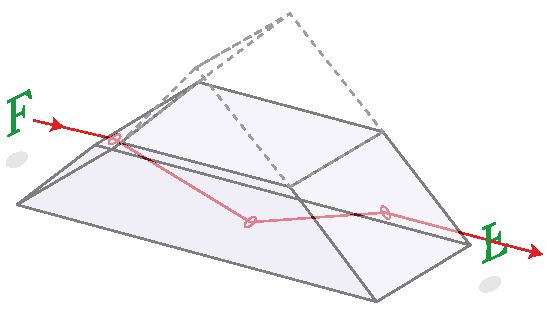
\includegraphics[width=0.5\textwidth]{dove-prism.pdf}
			\caption{达夫棱镜}
			\label{fig:dove-prism}
		\end{figure}
	\end{enumerate}
	\item \textbf{二次反射棱镜:}有两个反射面,相当于一个双面镜。夹角为$\alpha$的二次反射棱镜使光轴转过$2\alpha$角。
	\begin{enumerate}
		\item 五角棱镜
		\item 半五角棱镜
		\item 二次反射直角棱镜
		\item $30^{\circ}$直角棱镜
		\item 斜方棱镜
	\end{enumerate}
	\item \textbf{三次反射棱镜:}施密特棱镜,出射光轴相对于入射光轴改变了$45^{\circ}$方向。
\end{enumerate}

\subsection{屋脊棱镜}

\begin{definition}{屋脊棱镜}{roof-prism}
	将普通棱镜的一个反射面用两个互成直角的反射面替代的棱镜即为屋脊棱镜。两直角面的交线为棱线,平行于原反射面,且在主截面上。奇数次反射棱镜,用屋脊面代替其中一个反射面后,就成为了偶数次反射的屋脊棱镜。
\end{definition}

常见的屋脊棱镜有:屋脊直角棱镜、屋脊半五角棱镜、脊棱五角屋镜、屋脊施密特棱镜。

\subsection{角锥棱镜}
角锥棱镜具有三个互成直角的反射面,出射光线方向为入射光线的反方向。

\subsection{棱镜组合}

\begin{figure}[htbp]
	\centering
	\begin{minipage}[t]{0.45\textwidth}
		\centering
		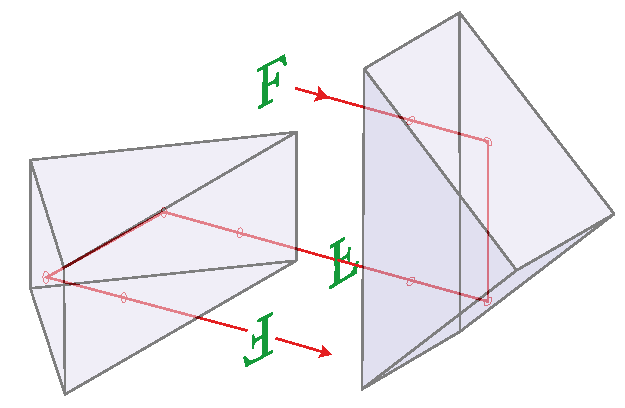
\includegraphics[width=1\textwidth]{double-porro-prism.pdf}
		\caption{普罗棱镜}
		\label{fig:double-porro-prism}
	\end{minipage}
	\qquad
	\begin{minipage}[t]{0.45\textwidth}
		\centering
		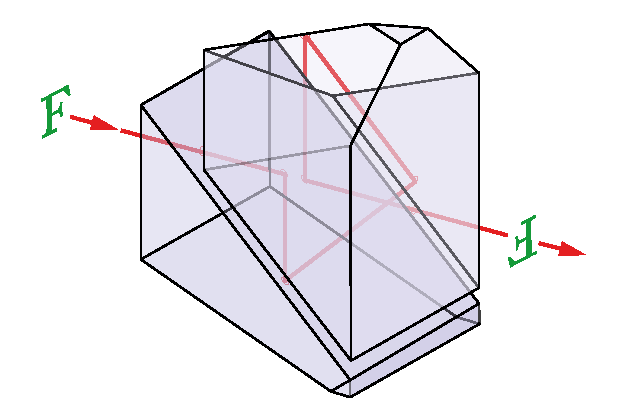
\includegraphics[width=1\textwidth]{schmidt-pechan-prism.pdf}
		\caption{别汉棱镜}
		\label{fig:schmidt-pechan-prism}
	\end{minipage}
\end{figure}

\begin{enumerate}
	\item 普罗棱镜(双普罗棱镜):如\figref{fig:double-porro-prism},由两块相同的等腰直角棱镜组成。
	\item 别汉棱镜(施密特-别汉棱镜组):如\figref{fig:schmidt-pechan-prism},由一块半五角棱镜和一块屋脊施密特棱镜、或一块屋脊半五角棱镜和一块施密特棱镜组成。特点为出射光轴的方向与入射光轴相同,可以让影像做$180^{\circ}$的旋转。
\end{enumerate}

\begin{problem}
	以下棱镜或棱镜组中哪些是成镜像的?
	\begin{tasks}(3)
		\task 别汉棱镜组
		\task 施密特棱镜
		\task 屋脊施密特棱镜
		\task 屋脊五角棱镜
		\task* 一次反射等腰直角棱镜与达夫棱镜的组合
	\end{tasks}
\end{problem}
\begin{solution}
	选择b和d。
\end{solution}

\begin{problem}
	以下光学系统中,可以成镜像的是:
	\begin{tasks}(3)
		\task 平面镜
		\task 别汉棱镜组
		\task 施密特棱镜
		\task 普罗型棱镜组
		\task 屋脊五角棱镜
	\end{tasks}
\end{problem}
\begin{solution}
	选择a、c和e。
\end{solution}

\section{折射棱镜}

\begin{figure}[htbp]
	\centering
	\begin{tikzpicture} 
	\coordinate (A) at (-2,0);
	\coordinate (B) at (0,3.464);
	\coordinate (C) at (2,0);
	\coordinate (D) at (1,1.732);
	\coordinate (E) at (0,1.155);
	\coordinate (F) at (2,2.309);
	\coordinate (G) at (-1.5,0.866);
	\coordinate (H) at (3,3.464);
	\coordinate (I) at (-3,0);
	\coordinate (J) at (-3,1.732);
	\coordinate (K) at (-0.5,0.289);
	\coordinate (L) at (0,1.732);
	\coordinate (M) at (3,1.732);
	\draw[-] (A) -- (B) -- (C) -- (A);
	\draw[-] (E) -- (F);
	\draw[-,dashed] (H) -- (G);
	\draw[-latex,red] (I) -- (G);
	\draw[-latex,red] (G) -- (D);
	\draw[-] (J) -- (K);
	\draw[-,dashed] (L) -- (D);
	\draw[-latex,red] (D) -- (M);
	\pic["$\alpha$", draw=black, -, angle eccentricity=1.4, angle radius=0.4cm] {angle=A--B--C};
	\pic[draw=black, -, angle radius=0.8cm] {angle=D--G--H};
	\pic["$\delta_2$", draw=black, -, angle eccentricity=1.6, angle radius=0.5cm] {angle=L--D--G};
	\pic["$\delta$", draw=black, latex-, angle eccentricity=1.1, angle radius=2.5cm] {angle=M--L--H};
	\pic["$I_1$", draw=black, -, angle eccentricity=1.6, angle radius=0.3cm] {angle=J--G--I};
	\pic["$I'_1$", draw=black, -, angle eccentricity=1.6, angle radius=0.3cm] {angle=K--G--D};
	\pic[draw=black, -, angle radius=0.9cm] {angle=G--D--E};
	\pic["$-I'_2$", draw=black, -, angle eccentricity=1.6, angle radius=0.5cm] {angle=M--D--F};
	\coordinate [label=above:$\delta_1$](delta-1) at (-1,1.1);
	\coordinate [label=below:$-I_2$](i-2) at (0.4,1.4);
	\coordinate [label=above:$n$](n) at (0,0.2);
	\end{tikzpicture}
	\caption{折射棱镜}
	\label{fig:refracting-prism}
\end{figure}

\figref{fig:refracting-prism} 画出了主截面内光线经过棱镜两个折射面折射后的情况。光线偏角为$\delta$,其正负规定为:由入射光线从锐角方向转到出射光线,顺时针为正,反之为负。对两个折射面写出折射定律:
\begin{equation}
\sin I_1=n\sin I'_1,\quad
\sin I'_2=n\sin I_2
\end{equation}
由\figref{fig:refracting-prism} 可得
\begin{equation}
\alpha=I'_1-I_2,\quad\delta=\delta_1+\delta_2=T_1-I'_1+I_2-I'_2
\end{equation}
从而
\begin{equation}
\alpha+\delta=I_1-I'_2
\end{equation}
综合上述公式得到
\begin{equation}
\sin\bigg(\frac{\alpha+\delta}{2}\bigg)=n\sin\frac{\alpha}{2}\cdot\frac{\cos\dfrac{I'_1+I_2}{2}}{\cos\dfrac{I_1+I'_2}{2}}
\end{equation}
当$\alpha$和$n$一定时,$\delta$仅随$I_1$而变。最小偏角与$\alpha$和$n$的关系为
\begin{equation}
\sin\bigg(\frac{\alpha+\delta_{\mathrm{min}}}{2}\bigg)=n\sin\frac{\alpha}{2}
\label{eq:minimum-deviation-angle}
\end{equation}

如果折射角很小,偏角公式分为两种情况:
\begin{enumerate}
	\item 光线入射角有一定大小,$I'_1=I_2$,$I_1=I'_2$,有
	\begin{equation}
	\delta=\alpha\bigg(\frac{n\cos I'_1}{\cos I_1}\bigg)
	\end{equation}
	\item 当光线垂直入射或入射角很小,有
	\begin{equation}
	\delta=\alpha(n-1)
	\end{equation}
\end{enumerate}

折射角很小的棱镜称为光楔。当双光楔绕光轴相对旋转,即一个光楔逆时针旋转$\varphi$角,另一个光楔顺时针旋转$\varphi$角,总偏角为$2\varphi$,有
\begin{equation}
\delta=2(n-1)\alpha\cos\frac{\varphi}{2}
\end{equation}

\begin{problem}
	有一等边折射三棱镜,其折射率为$1.65$,求光线经该棱镜的两个折射面折射后产生最小偏角时的入射角,并求出最小偏角值。
\end{problem}
\begin{solution}
	由\figref{fig:refracting-prism} 可知,当$I_1=-I'_2$时,产生最小偏角。由公式$\alpha+\delta=I_1-I'_2$可得,$I_1=55.6^{\circ}$。由式 (\ref{eq:minimum-deviation-angle}) 可得,最小偏角$\delta_m=51.2^{\circ}$。
\end{solution}

\section{光的色散}
以太阳光谱中的夫琅禾费谱线作为特征,单色谱线来表征光学介质的折射率,这些谱线的符号、颜色、波长以及产生谱线的元素如\tabref{tab:spectral-line} 所示。

\begin{table}[htbp]
	\small
	\centering
	\caption{各单色谱线的符号、颜色、波长以及产生谱线的元素}
	\begin{tabular}{c|c|c|c|c|c|c|c|c|c|c}
		\hline
		符号&$A'$&$b$&$C$&$D$&$d$&$e$&$F$&$g$&$G'$&$h$\\
		\hline
		颜色&\multicolumn{3}{c|}{红}&\multicolumn{2}{c|}{黄}&绿&\multicolumn{2}{c|}{青}&蓝&紫\\
		\hline
		$\lambda$(nm)&$768.2$&$706.5$&$656.3$&$589.3$&$587.6$&$546.1$&$486.1$&$435.8$&$434.0$&$404.7$\\
		\hline
		元素&K&He&H&Na&He&Hg&H&Hg&H&Hg\\
		\hline
	\end{tabular}
	\label{tab:spectral-line}
\end{table}

\section{光学材料}
\label{sect:optical-material}
光学玻璃可分为冕牌和火石两大类。冕牌玻璃低折射率低色散,火石玻璃高折射率高色散。阿贝常数$v_D$:
\begin{equation}
v_D=\frac{n_D-1}{n_F-n_C}
\end{equation}

\begin{property}
	阿贝常数越大,色散越低,反之,色散越大。
\end{property}

\begin{problem}
	某种光学玻璃d光的折射率为$1.51637$,$C$光的折射率为$1.51389$,阿贝常数为$64.1$,求$F$光的折射率。
	\begin{tasks}(2)
		\task $1.52196$
		\task $1.50583$
	\end{tasks}
\end{problem}
\begin{solution}
	选择a。
\end{solution}

\begin{problem}
	有一光楔,其材料为K9玻璃($n_F=1.52196$,$n_C=1.51389$),白光经其折射后要发生色散。若要求出射的F光和C光间的夹角$\delta_{F,C}<1'$,求光楔的最大折射角应为多少。
\end{problem}
\begin{solution}
	当光线垂直入射或入射角很小,有$\delta=\alpha(n-1)$。对于F光,出射光线的偏角为$\delta_F=\alpha(n_F-1)$;对于C光,出射光线的偏角为$\delta_C=\alpha(n_C-1)$。其夹角为$\delta_{FC}=\delta_F-\delta_C=\alpha(n_F-1)-\alpha(n_C-1)=0.00807\alpha$。要使$\delta_{FC}=0.00807\alpha<1'$,则有$\alpha=1'/0.00807=2^{\circ}4'4''$。即最大折射角为$2^{\circ}4'4''$。
\end{solution}